\documentclass[12pt,a4paper]{article}
%-------------------------------------------
%---Packages--------------------------------
%-------------------------------------------
\usepackage[utf8]{inputenc}
%\usepackage[T1]{fontenc}
%\usepackage{txfonts}
\usepackage{amsmath}
\usepackage{amsthm}
\usepackage{amsfonts}
\usepackage{array}
\usepackage{amssymb}
\usepackage{blindtext}
\usepackage{caption}
\usepackage{color}
\usepackage{csquotes}	    %
\usepackage{enumitem}	    %pour mieux bosser avec les listes. ajoute option label
\usepackage[yyyymmdd]{datetime}        %pour définir date custom
\usepackage{etaremune}
\usepackage{environ}
\usepackage{fancybox}
\usepackage{fancyhdr} 	    % Custom headers and footers
\usepackage{fancyref}
%\usepackage{float}
\usepackage{floatrow}       %float and floatrow can't be together...
\usepackage{gensymb}
\usepackage{graphicx}
\usepackage[colorlinks=true, linkcolor=purple, citecolor=cyan]{hyperref}
\usepackage{footnotebackref}
\usepackage{lipsum}
\usepackage{mathtools}
\usepackage{multicol}	    %gérer plusieurs colonnes
\usepackage{setspace}
\usepackage{subcaption}
\usepackage{todonotes}	    %Bonne gestion des TODOs
%TODO commenté pour tester l'utilité... à voir% \usepackage[tc]{titlepic}      %Permet de mettre une image en page de garde
\usepackage{tikz}	    % Pour outil de dessin puissant
\usepackage{ulem}	    %underline sur plusieurs lignes (avec \uline{})
\usepackage{vmargin} 	    %gestion des marges, avec dans l'ordre : gauche, haut, droit, bas, en-tête, entre en-tête et texte, bas de page, hauteur entre bas de page et texte
\usepackage{wrapfig}
\usepackage{xcolor}
\usepackage{xparse}                    %Pour utiliser NewDocumentCommand et des arguments 'mmooo'
%\usepackage{fullpage} 	    %supprime toutes les marges allouées aux notes, aussi en haut et en bas

%\ExplSyntaxOn
\pagestyle{fancyplain}	    %Makes all pages in the document conform to the custom headers and footers

%-------------------------------------------
%---Document Commands-----------------------
%---------------------------{----------------
\NewDocumentCommand{\framecolorbox}{oommm}
 {% #1 = width (optional)
  % #2 = inner alignment (optional)
  % #3 = frame color
  % #4 = background color
  % #5 = text
  \IfValueTF{#1}%
   {\IfValueTF{#2}%
    {\fcolorbox{#3}{#4}{\makebox[#1][#2]{#5}}}%
    {\fcolorbox{#3}{#4}{\makebox[#1]{#5}}}%
   }%
   {\fcolorbox{#3}{#4}{#5}}%
 }%
%------------------------------------------------
%------------------ENGLISH----------------------
%----------------------------------------------

\NewDocumentCommand{\epflTitle}{mO{Olivier Cloux}O{\today}O{Notes de Cours en}D<>{../../Common}}%Arguments : Matière, Auteur, Date, Titre du doc
{
\begin{titlepage}
    \vspace*{\fill}
    \begin{center}
        \normalfont \normalsize
        \textsc{Ecole Polytechnique Fédérale de Lausanne} \\ [25pt] % Your university, school and/or department name(s)
        \textsc{#4} %Titre du doc
        \\ [0.4 pt]
        \horrule{0.5pt} \\[0.4cm] % Thin top horizontal rule
        \huge #1 \\ % Matière
        \horrule{2pt} \\[0.5cm] % Thick bottom horizontal rule
        
\includegraphics[width=8cm]{#5/EPFL_logo}
        ~\\[0.5 cm]
        \small\textsc{#2}\\[0.4cm]
        \small\textsc{#3}\\
        ~\\
        ~\\
        
\includegraphics[scale=0.5]{#5/creativeCommons}
    \end{center}
    \vspace*{\fill}
\end{titlepage}
}


%-------------------------------------------
%-------------MATH NEW COMMANDS-------------
%-------------------------------------------
\newcommand{\somme}[2]{\ensuremath{\sum\limits_{#2}^{#1}}}
\newcommand{\produit}[2]{\ensuremath{\prod\limits_{#2}^{#1}}}
\newcommand{\limite}{\lim\limits_}
\newcommand{\llimite}[3]{\limite{\substack{#1 \\ #2}}\left(#3\right)}	%limites à deux condiitons
\newcommand{\et}{\mbox{ et }}
\newcommand{\deriv}[1]{\ensuremath{\, \mathrm d #1}}	%sigle dx, dt,dy... des dérivées/intégrales
%\newcommand{\fx}{\ensuremath{f'(\textbf{x}_0 + h}}
\newcommand{\ninf}{\ensuremath{n \to \infty}}	       %pour les limites : n tend vers l'infini
\newcommand{\xinf}{\ensuremath{x \to \infty}}	       %pour les limites : x tend vers l'infini
\newcommand{\infint}{\ensuremath{\int_{-\infty}^{\infty}}}
\newcommand{\xo}{\ensuremath{x \to 0}}									%x to 0
\newcommand{\no}{\ensuremath{n \to 0}}									%n zéro
\newcommand{\xx}{\ensuremath{x \to x}}									%x to x
\newcommand{\Xo}{\ensuremath{x_0}}										%x zéro
\newcommand{\X}{\ensuremath{\mathbf{X}} }
\newcommand{\A}{\ensuremath{\mathbf{A}} }
\newcommand{\R}{\ensuremath{\mathbb{R}} }								%ensemble de R
\newcommand{\rn}{\ensuremath{\mathbb{R}^n} } 							%ensemble de R de taille n
\newcommand{\Rm}{\ensuremath{\mathbb{R}^m} }  							%ensemble de R de taille m
\newcommand{\C}{\ensuremath{\mathbb{C}} }
\newcommand{\N}{\ensuremath{\mathbb{N}} }
\newcommand{\Z}{\ensuremath{\mathbb{Z}} }
\newcommand{\Q}{\ensuremath{\mathbb{Q}} }
\newcommand{\rtor}{\ensuremath{\R \to \R} }
\newcommand{\pour}{\mbox{ pour }}
\newcommand{\coss}[1]{\ensuremath{\cos\(#1\)}}						%cosinus avec des parenthèses de bonne taille (genre frac)
\newcommand{\sinn}[1]{\ensuremath{\sin\(#1\)}}					%sinus avec des parentèses de bonne taille (genre frac)
\newcommand{\txtfrac}[2]{\ensuremath{\frac{\text{#1}}{\text{#2}}}}		%Fractions composées de texte
\newcommand{\evalfrac}[3]{\ensuremath{\left.\frac{#1}{#2}\right|_{#3}}}
\renewcommand{\(}{\left(}												%Parenthèse gauche de taille adaptive
\renewcommand{\)}{\right)}
\newcommand{\longeq}{=\joinrel=}												%Parenthèse droite de taille adaptive


%-------------------------------------------------------
%------------------MISC NEW COMMANDS--------------------
%-------------------------------------------------------
\newcommand{\degre}{\ensuremath{^\circ}}
%\newdateformat{\eudate}{\THEYEAR-\twodigit{\THEMONTH}-\twodigit{\THEDAY}}



%-------------------------------------------------------
%------------------TEXT NEW COMMANDS--------------------
%-------------------------------------------------------
\newcommand{\ts}{\textsuperscript}
\newcommand{\evid}[1]{\textbf{\uline{#1}}}        %mise en évidence (gras + souligné)



%\newcommand{\Exemple}{\underline{Exemple}}
\newcommand{\Theoreme}{\underline{Théorème}}
\newcommand{\Remarque}{\underline{Remarque}}
\newcommand{\Definition}{\underline{Définition} }
\newcommand{\skinf}{\sum^{\infty}_{k=0}}
\newcommand{\combi}[2]{\ensuremath{\begin{pmatrix} #1 \\ #2 \end{pmatrix}}}	%combinaison parmi 1 de 2
\newcommand{\intx}[3]{\ensuremath{\int_{#1}^{#2} #3 \deriv{x}}}				%intégrale dx
\newcommand{\intt}[3]{\ensuremath{\int_{#1}^{#2} #3 \deriv{t}}}				%intégrale dy
\newcommand{\misenforme}{\begin{center} Mis en forme jusqu'ici\\ \line(1,0){400}\\ normalement juste, mais à améliorer depuis ici\end{center}}	%raccourci pour mise en forme
\newcommand*\circled[1]{\tikz[baseline=(char.base)]{
            \node[shape=circle,draw,inner sep=1pt] (char) {#1};}}			%pour entourer un chiffre
\newcommand{\horrule}[1]{\rule{\linewidth}{#1}} 				% Create horizontal rule command with 1 argument of height

\theoremstyle{definition}
\newtheorem{exemp}{Exemple}
\newtheorem{examp}{Example}


%-------------------------------------------
%---Environments----------------------------
%-------------------------------------------
\NewEnviron{boite}[1][0.9]{%
	\begin{center}
		\framecolorbox{red}{white}{%
			\begin{minipage}{#1\textwidth}
 	 			\BODY
			\end{minipage}
		}
	\end{center}
}
\NewEnviron{blackbox}[1][0.9]{%
	\begin{center}
		\framecolorbox{black}{white}{%
			\begin{minipage}{#1\textwidth}
 	 			\BODY
			\end{minipage}
		}
	\end{center}
}
\NewEnviron{exemple}[1][0.8]{%
    \begin{center}
        \framecolorbox{white}{gray!20}{%
            \begin{minipage}{#1\textwidth}
                \begin{exemp}
                    \BODY
                \end{exemp}
            \end{minipage}
        }
    \end{center}
}
\NewEnviron{suiteExemple}[1][0.8]{%
    \begin{center}
        \framecolorbox{white}{gray!20}{%
            \begin{minipage}{#1\textwidth}
                \BODY
            \end{minipage}
        }
    \end{center}
}
\NewEnviron{colExemple}[1][0.8]{%
    \begin{center}
        \framecolorbox{white}{gray!20}{%
            \begin{minipage}{#1\columnwidth}
                \begin{exemp}
                    \BODY
                \end{exemp}
            \end{minipage}
        }
    \end{center}
}
\NewEnviron{example}[1][0.8]{%
    \begin{center}
        \framecolorbox{white}{gray!20}{%
            \begin{minipage}{#1\textwidth}
                \begin{examp}
                    \BODY
                \end{examp}
            \end{minipage}
	}
    \end{center}
}
\NewEnviron{systeq}[1][l]{
			\begin{center}
				$\left\{\begin{array}{#1}
					\BODY
				\end{array}\right.$
			\end{center}
 }





%-------------------------------------------
%---General settings-----------------------
%-------------------------------------------
\renewcommand{\headrulewidth}{1pt}										%ligne au haut de chaque page
\renewcommand{\footrulewidth}{1pt}										%ligne au pied de chaque page
\setstretch{1.6}
\author{Olivier Cloux}

\usepackage{framed}
\setstretch{1}
\title{	
\normalfont \normalsize 
\textsc{Ecole Polytechnique Fédérale de Lausanne} \\ [25pt] % Your university, school and/or department name(s)
\horrule{0.5pt} \\[0.4cm] % Thin top horizontal rule
\huge Résumé d'Analyse II\\ % The assignment title
\horrule{2pt} \\[0.5cm] % Thick bottom horizontal rule
}
\setmarginsrb{15mm}{15mm}{15mm}{15mm}{-5pt}{15mm}{0pt}{8mm}
\date{Printemps 2015}
\setcounter{section}{-1}
\newlength\tindent
\setlength{\tindent}{\parindent}
%\setlength{\parindent}{0pt}
\renewcommand{\)}{\right)}
\renewcommand{\(}{\left(}
\setstretch{1}
\begin{document}
\maketitle
\section{Rappels}
\subsection{Autre}
\begin{itemize}
	\item 	Équation d'un cercle de rayon $=r$ et de centre $=(a,b) \to (x-a)^2 + (y-b)^2 = r^2$
	\item	Équation d'une sphère de rayon $=r$ et de centre $=(a,b,c) \to (x-a)^2 + (y-b)^2 + (z-c)^2 = r^2$
\end{itemize}
\subsection{Périodicité}
\begin{itemize}
	\item Le produit (et la somme) de deux fonctions périodique est périodique si le rapport des périodes est rationnel. $\frac{T_f}{T_g} \in \Q \to \frac{T_f}{T_g} = \frac{r}{s} \iff T = T_f\cdot s = T_g\cdot r$
	\item La composition d'une fonction quelconque avec une fonction périodique est périodique. $h\circ f$ est $T_f$ périodique
\end{itemize}
\subsection{Trigonométrie}
\begin{itemize}
	\item $1+\cos(2x) = 2\cos^2(x)$
	\item $1-\cos(2x) = 2\sin^2(x)$
	\item $\cos(x)\sin(x) = \frac{1}{2}\sin(2x)$
	\item $\sin^2(x)+\cos^2(x) = 1 \iff \sin^2(x) = 1-\cos^2(x) \iff \cos^2(x) = 1-\sin^2(x)$
	\item $\frac{1}{cos} = \frac{1}{\sqrt{1-\sin^2(x)}}$ (pratique, car $\intx{}{}{\frac{1}{\sqrt{1-x^2}}} = \arcsin(x)$
\end{itemize}
<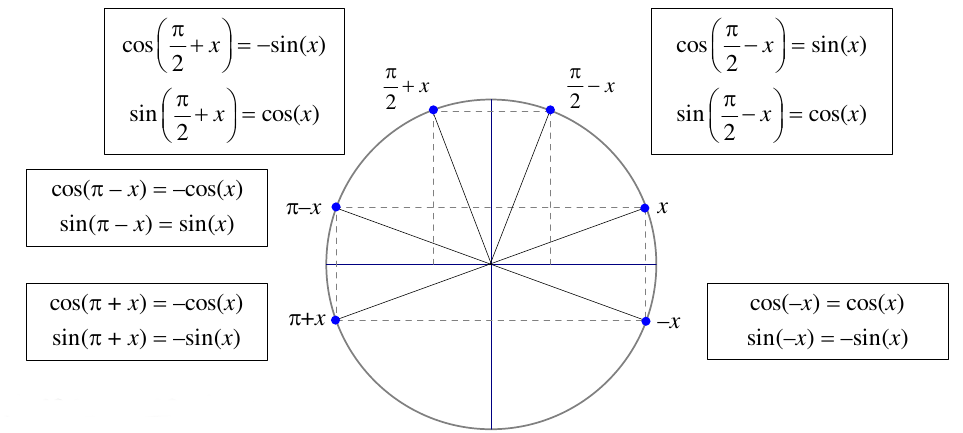
\includegraphics[scale=0.5]{trigo}\\
\begin{tabular}{c|c|c|c|c}
Degrés & Radians & SINUS & COSINUS & TANGENTE\\
\hline
$0$ & $0$ & $\frac{\sqrt{0}}{2}$ & $\frac{\sqrt{4}}{2}$ & $0$\\
\hline
$30$ & $\frac{\pi}{6}$ & $\frac{\sqrt{1}}{2}$ & $\frac{\sqrt{3}}{2}$ & $\frac{1}{\sqrt{3}}$\\
\hline
$45$ & $\frac{\pi}{4}$ & $\frac{\sqrt{2}}{2}$ & $\frac{\sqrt{2}}{2}$ & $1$\\
\hline
$60$ & $\frac{\pi}{3}$ & $\frac{\sqrt{3}}{2}$ & $\frac{\sqrt{1}}{2}$ & $\sqrt{3}$\\
\hline
$90$ & $\frac{\pi}{2}$ & $\frac{\sqrt{4}}{2}$ & $\frac{\sqrt{0	}}{2}$ & $\infty$\\

\end{tabular}
\subsection{Intégration}
\begin{itemize}
	\item 	$\intx{}{}{\frac{1}{\sqrt{x^2+1}}} = \sinh^{-1}(x)$ (arcsinh)
	\item 	$\intx{}{}{\frac{f'(x)}{1+f(x)^2}} = \arctan(f(x)$ Notons aussi que $\int \frac{1}{t^2 + x^2} \deriv{x} = \frac{1}{t}\arctan\(\frac{x}{t}\)$
	\item 	$\int\frac{1}{\sqrt{1-x^2}} \deriv{x} = \arcsin(x)$
	\item 	$\int-\frac{1}{\sqrt{1-x^2}}\deriv{x} = \arccos(x)$
\end{itemize}
\subsubsection{Intégration par changement de variable}
Nous avons une intégrale de la forme $\intx{a}{b}{f(x)}$. La formule est :
\begin{equation*}
	\intx{a}{b}{f(x)} = \int_\alpha^\beta f(\varphi(u)) \varphi'(u) \, du
\end{equation*}
Donc:
\begin{enumerate}
	\item Choisir un $\varphi(u)$ qui "annule" un bout de la fonction qui nous embête. Si on a un $\sqrt{x}$, il est bon de placer $x = f(u) = u^2$, ce qui donnera $\sqrt{x} = \sqrt{u^2} = u$
	\item On calcule la dérivée de $\varphi(u)$
	\item On calcul les bornes : on cherche $\alpha, \beta$ tels que $\varphi(\alpha) = a$ (et b)
	\item Assembler le tout pour correspondre à l'équation au dessus
\end{enumerate}
\subsubsection{Intégration par partie}
\begin{equation*}
	\intx{a}{b}{f(x)g(x)} = [F(x)g(x)]_a^b - \intx{a}{b}{F(x)g'(x)}
\end{equation*}
\begin{enumerate}
	\item (note : si pas de bornes, on enlève juste les bornes)
	\item Choisir une fonction \enquote{grandissante} (à intégrer) et une \enquote{descendante} (à dériver).
	\item Faire l'opération une fois. On peut répéter pour la seconde partie
	\item À utiliser avec des fonctions \enquote{périodiques} (cos, sin, $e^x$,\ldots, car une seconde fois nous ramène sur l'opération initiale
	\item On peut donc des fois faire une double intégration et trouver $\int f(x) = g(x) - \int f(x)$, ce qui nous permet de trouver $2\int f(x) = g(x) \iff \int f(x) = \frac{g(x)}{2}$
\end{enumerate}

\subsubsection{Décomposition en éléments simples}
\label{elements simples}
Très utile pour intégrer des fractions. On choisit des A,B,... pour lesquels on peut additionner les termes qui avant se multipliaient
\begin{exemple}[0.9]
\[\frac{\deriv{y}}{\deriv{x}} = y(a-by) \iff \frac{1}{y(a-by)}dy = dx \iff \int\frac{1}{y(a-by)}dy = \int \deriv{x}\] Depuis là, on décompose le terme de gauche en éléments simples : On suppose qu'il existe un A et un B tels que
\begin{align*}
	\frac{A}{y} + \frac{B}{a-by} = \frac{1}{y(a-by)} \iff \frac{A(a-by) + By}{y(a-by)} = \frac{1}{y(a-by)}\\
	 \iff A(a-by) + By = 1 \iff y(B -Ab) +Aa = 1
\end{align*}
On analyse les termes en $y$, en $y^2$, en \enquote{1},...(ici que $y$ et 1)
\begin{itemize}
	\item[1] $Aa = 1 \iff A = \frac{1}{a}$
	\item[y] $B-Ab = B-\frac{1}{a}b = 0 \iff B = \frac{a}{b}$
\end{itemize}
On peut donc réécrire notre intégrale comme $\int \frac{1}{y(a-by)} = \int \frac{1}{ay} \deriv{y} + \int \frac{b}{a(a-by)} \deriv{y} = \frac{1}{a}\ln(|y|) - \frac{1}{a}\ln(|a-by|)$
\end{exemple}


\subsection{Dérivées}
Une fonction est dérivable en un point si $\frac{f(x) - f(x_0)}{x-x_0}$ avec $x_0$ le point analysé, celui qui peut embêter.
\begin{itemize}
	\item $(a^x)' = a^x\ln(a)$
	\item $f(x) = g(x)^{h(x)} = e^{h(x) \ln(g(x))} \to f'(x) = e^{h(x)\ln(g(x))}\left(h'(x)\ln(g(x)) + g'(x)\frac{1}{g(x)}h(x)\right)$
\end{itemize}
\subsection{Algèbre linéaire}
\begin{itemize}
	\item 	Inverser une matrice de la forme 
			$\begin{pmatrix}
				A & B\\
				C & D
			\end{pmatrix}$ : On cherche d'abord le déterminant, puis on change la matrice de forme, pour obtenir :
			\begin{equation*}
				\frac{1}{\det(M)} \begin{pmatrix}
				D & -B\\
				-C & A
				\end{pmatrix} \qquad \det(M) = (AD-BC)
			\end{equation*}
	\item 	Diagonalisation. Pour une matrice A, il peut exister (entre autres si elle est symétrique) deux matrices $V,D$ telles que $A = VDV^T$. Nous devons simplement chercher les vecteurs propres (calculer $det(A-\lambda I)$) pour trouver nos valeurs propres (à mettre dans la diagonale de D), puis, pour chaque $\lambda$, résoudre $Av = \lambda v$ et trouver ainsi autant de vecteurs propres, à normaliser (diviser par leur norme) puis mettre dans V aux positions correspondant aux valeurs propres (en mettant $\lambda_1$ dans la colonne 1, puis trouvant la valeur propre associée, il faut mettre $v_1$ en première colonne de V)
\end{itemize}

\subsection{Limites}
\begin{itemize}
	\item $\limite{x\to 0} x\ln(|x|) = 0$ (on change en $\frac{ln(x)}{\frac{1}{x}}$, BH, on dérive, =x = 0)
\end{itemize}
\subsection{Analyse I}
\subsubsection{Continuité}
Une fonction est continue en $x_0 = l$ si $\limite{x\to x_0}{f(x)} = l$.\\
Par exemple, $f(x) = 
\left\{\begin{array}{ll}
	\frac{\sin(x)}{x} & x\neq 0\\
	1 & x = 0
\end{array}\right.$ On analyse si lorsqu'on tend vers 0, la fonction donne 1. Après vérification, on voit que c'est égal. Donc la fonction est continue en $x=0$ (et on voit qu'elle est continue ailleurs)
\section{ED ordre 1}
\subsection{Notation, appellations, définitions,\ldots}
\begin{itemize}
	\item Ordre : plus grande dérivée ($y''+y'+3 = 0 \to$ ordre 2, car dérivée seconde).
	\item Degré : puissance de la \underline{plus grande} dérivée ($(y'')^{2} + (y')^{4} + y^{10} + 100$ degré 2)
	\item Donc une ED linéaire d'ordre 1 est de la forme : $E(x,y,y') = f(x) -g(y)y' = 0$
	\item Maximale : On dit qu'une solution est maximale si elle n'est pas la restriction d'une autres solution. Se trouve en général avec des conditions initiales.
\end{itemize}

\subsection{Séparation des variables}
Une ED est dite à variables séparées si on peut l'écrire sous la forme
\[E(x,y,y') = f(x) - g(y)y' = 0 \iff f(x) = g(y)y'\]
Pour résoudre une équation de degré 1, il faut déjà essayer par intégration : si elle est simple ($y''=0$) il est facile de simplement intégrer. \\
Si il est impossible de le faire simplement, on tente de :
\begin{enumerate}
	\item Réécrire notre ED sous la forme $f(x)-g(y)y'$
	\item Remplacer $y'$ par $\frac{\deriv{y}}{\deriv{x}}$, et réécrire l'équation.
	\item Séparer $f(x)$ et $g(y)$, pour obtenir quelque chose de la forme \\$g(y)\deriv{y} = f(x)\deriv{x}$
	\item Intégrer des deux côtés, avec une (et une seule\footnote{car si deux, elles vont se \enquote{fondre} en une seule}) constante.
\end{enumerate}

On peut aussi aller à la manière \enquote{homogène + particulière} (dans un sens). On trouve souvent une solution particulière (genre $y(x) = 2$) donc on devrait trouver un +2 à la fin. Il faut de toute manière s'assurer qu'il existe un C tel que la solution particulière qu'on a trouvé  est possible.\\
\\
\begin{exemple}
	\begin{align*} 
	y' = -xy \iff y'\frac{1}{y} = -x \iff \frac{\deriv{y}}{\deriv{x}} \frac{1}{y} = -x \iff \frac{1}{y}\deriv{y} = -x \deriv{x} \quad |\int\\
	\iff\ln(|y|) = -\frac{1}{2}x^2 + C \iff y(x)=e^{-\frac{x^2}{2} + C} = e^{-\frac{x^2}{2}} \cdot \underbrace{e^C}_{=C} = Ce^{-\frac{x^2}{2}}
	\end{align*}
	Si $C = 0,\ y(x) = 0 \to$ condition respectée\\
	$\to$ Solution générale : $y(x) = Ce^{-\frac{x^2}{2}}$
\end{exemple}

\begin{exemple}
	Prenons l'ED 
	\[y' = 2y(5-y)\]
	Nous pouvons faire comme nous savons, a savoir 
	\begin{equation}
	\frac{\deriv{y}}{\deriv{y}} = 2y(5-y) \iff \frac{1}{2y(5-y)} \deriv{y} = 1\deriv{x}
	\label{separation variables exemple}
	\end{equation}
	Mais attention ! En faisant ça, nous avons ôté deux possibilités, celles ou $y = 0$ et $y = 5$ (auquel cas 1/0). Nous devons donc affirmer au début que $y=0$ et $y = 5$ sont des solutions (et du coup $y' = 0$). Ensuite nous regardons l'ED \textit{dans le cas où $y \neq 0$ et $y \neq 5$}. Une fois cette \enquote{formalité} passée, nous pouvons passer à la suite, c'est à dire utiliser la \hyperref[elements simples]{décomposition en éléments simples} pour faciliter l'intégration : 
	\begin{align*}
	\frac{1}{2y(5-y)} = \frac{A}{2y} + \frac{B}{5-y} = \frac{A(5-y) + B(2y)}{2y(5-y)} \to y(2B-A)  + 5A = 1\\
	\to
	\left\{ \begin{array}{l}
	2B-A = 0\\
	5A = 1
	\end{array}\right. \to A = \frac{1}{5}\quad B =\frac{1}{10}
	\end{align*}
	On peut donc réécrire notre équation de base :
	\begin{align*}
		\frac{1}{2y(5-y)} = \frac{1}{10y} + \frac{1}{10(5-y)} = \frac{1}{10}\(\frac{1}{y} + \frac{1}{5-y}\)
	\end{align*}
	Après intégration des deux côtés de \eqref{separation variables exemple} on obtient 
	\begin{align*}
		\frac{1}{10}(\ln|y| + \ln|5-y|) = x + C \iff \ln\left|\frac{y}{5-y}\right| = 10(x + C) = 10x + C\\
		\iff \frac{y}{5-y} = \pm e^{10x + C} = \pm Ce^{10x} \iff y(x) = \frac{5Ce^{10x}}{1+Ce^{10x}}
	\end{align*}
	ce qui est la solution générale. Le dernier point consiste en l'expression des ensembles de définition. Il faut noter là que si $C > 0$, alors $x$ peut prendre toutes les formes. En revanche, si $C < 0$, alors $y(x)$ n'est solution que pour $x \in ]-\infty,-\frac{1}{10 \ln(-C)}[$ ou $x\in ]-\frac{1}{10}\ln(-C),\infty[$, ce qui se résume par le tableau à la Figure \ref{tab separation variables}
\end{exemple}
\begin{figure}[!h]
	\centering
	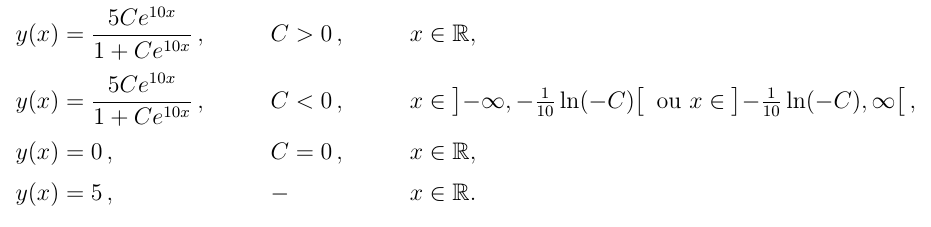
\includegraphics[scale=0.5]{separation_variable}
	\caption{}
	\label{tab separation variables}
\end{figure}
\subsection{Linéaires}
De la forme $y' + p(x)y = q(x).\qquad q(x) = 0$ homogène
\subsubsection{Résolution}
Une telle résolution se fait en 2 parties : d'abord résoudre l'équation homogène (on place $q(x) = 0$), puis trouver une solution particulière.
\begin{enumerate}
	\item Prendre l'équation homogène associée $(\to q(x) = 0$)
	\item Chercher la solution homogène \fbox{$y_0$}:
		\begin{enumerate}
			\item Faire comme avant, mode \enquote{recette de cuisine}. Il faut traiter $\frac{\deriv{y}}{\deriv{x}}$ comme une fraction.
			\item En travaillant l'équation un peu avant, on se trouve avec quelque chose du type \fcolorbox{red}{white}{$y_0(x) = e^{-P(x)}$}
		\end{enumerate}
	\item Chercher la solution particulière \fbox{$y_p(x)$}
		\begin{itemize}
			\item Façon Variation de la constante :
				\begin{enumerate}
					\item $y_p(x) = C(x)y_0(x) \to y_p'(x) = C'(x)y_0(x) + C(x)y_0'(x)$
					\item $y_p'(x) + p(x)y_p(x) = C'(x)y_0(x) + \underbrace{C(x)y_0'(x) + p(x)C(x)y_0(x)}_{= C(x)\big(y_0'(x) + p(x)y_0(x)\big) = 0}$
					\item $y_p'(x) = C'(x)y_0(x) = q(x) \iff C'(x) = \frac{1}{y_0(x)}q(x) = e^{P(x)}q(x)$
					\item $\to y_p(x) = \left(\intx{}{}{e^{P(x)}q(x)}\right)e^{-P(x)}$
				\end{enumerate}
			\item Façon C\oe fficients indéterminés
				\begin{enumerate}
					\item Ne s'applique que si $p(x) = const$ et si $q(x)$ est fonction polynôme, exponentielle, sin, cos, produit de tout ça.
					\item On pose $y_p(x) = C_1q(x) + C_2q'(x) + C_3q''(x) + ...$, avec autant de dérivées qu'il y en a de différentes (par exemple, $q(x) = \cos(x)$, alors on prendra $q(x)$ et $q'(x)$, car $q''(x) = q(x)$ à un facteur près. Si une dérivée est solution de l'équation, (donc $y(x) = q^{(n)}(x)$ fonctionne) alors il faut placer $Cxq^{(n)}(x)$
					\item Ensuite on fait ce qu'il faut (chercher $y_p'$ souvent) pour pouvoir la mettre dans l'ED de départ, et donc trouver $C_{1,2}$
				\end{enumerate}
		\end{itemize}
	\item Finalement, la solution générale \fbox{$y(x) = y_p(x) + Cy_0(x)$}
\end{enumerate}

\begin{exemple}
\setstretch{1}
	$y' -y\sin(x) = 4\sin(x=e^{\cos(x)}$\\
	\\
	\underline{1\ts{ère} étape : Trouver la solution  générale :}\\
	$\begin{array}{lr}
		y' -y\sin(x) = 0  & \text{solution homogène}\\
		y_h = Ce^{\int\sin(x)\deriv{x}} = Ce^{-\cos(x)} & \text{selon théorie, et vu au dessus}\\
	\end{array}$\\
	\\
	\underline{2\ts{ème} étape : trouver la solution particulière}\\
	$\begin{array}{ll}
		y_p = C(x)e^{-\cos(x)}\\
		y'_p = \big(C'(x) + \sin(x)C(x)\big)e^{-\cos(x)}
	\end{array}$\\
	On remplace $y$ et $y'$ dans l'équation originelle\\
	$\begin{array}{l}
		 \big(C'(x) + \sin(x)C(x)\big)e^{-\cos(x)} - C(x)e^{-\cos(x)}\sin(x) = 4\sin(x)e^{\cos(x)}\\
		 \iff C'(x)e^{-\cos(x)} = 4\sin(x)e^{\cos(x)}\\
		 \iff C'(x) = 4\sin(x)e^{2\cos(x)}\\
		 \iff C(x) = 2e^{2\cos(x)}
	\end{array}$\\	
	On rentre le $C(x)$ dans notre $y_p$\\
	$\to y_p(x) = -2e^{2\cos(x)}e^{-\cos(x)}\\
	= 2e^{\cos(x)}$\\
	\\
	\underline{Finalement, on additionne $y_h$ et $y_p$}\\
	$\to y(x) = y_h(x) + y_p(x) = Ce^{-\cos(x)} -2e^{\cos(x)}$
\end{exemple}
\subsection{Problème de Cauchy} 	
Une équation est un problème de Cauchy quand nous avons une conditions initiale à respecter. Nous devons donc chercher la solution général ($y = y_h + y_p$), puis ajouter la dedans nos conditions (par exemple, $y(3) = 0$ signifie qu'en remplaçant tous les x par 3, le total sera =0). En général nous avons une condition par constante $C_\alpha$.
\section{Ordre 2}
m\subsection{ED linéaires du deuxième ordre à coefficients constants}
Équation du type \fbox{$ay''+by'+cy = q(x)$}\\
On cherche aussi la solution homogène et la solution particulière, pour les additionner. Si $q(x) = 0$, il n'y a pas de solution particulière (qu'une solution homogène).
\subsubsection{Résolution de $y_h$}
L'équation sera forcément de la forme $y_h(x) = C_1y_1(x) + C_2y_2(x)$\\
La résolution se fait comme une équation du second degré. On utilise la méthode de résolution $\frac{-b \pm \sqrt{b^2-4ac}}{2a}$, qui peut déboucher sur trois cas :
\begin{itemize}
	\item[$>0$: ]	Si $b^2-4ac > 0$, on obtient deux solutions $\lambda_1,\lambda_2$, qui iront dans la solution homogène
					\begin{equation*}
						y_h(x) = C_1e^{\lambda_1 x} + C_2e^{\lambda_2 x}
					\end{equation*}
	\item[$=0$: ]	Si $b^2-4ac = 0$, nous obtenons une seule solution $\lambda$, qui ira dans la solution homogène 
					\begin{equation*}
						y_h(x) = C_1e^{\lambda x} + C_2xe^{\lambda x}
					\end{equation*}
	\item[$<0$: ]	Si $b^2-4ac < 0$, nous obtenons deux solution $\lambda, \overline{\lambda}$ (avec $\lambda = \alpha + \beta i$). Elles iront dans la solution homogène
					\begin{equation*}
						y_h(x) = C_1e^{\alpha x}\cos(\beta x) + C_2e^{\alpha x}\sin(\beta x)
					\end{equation*}
\end{itemize}
\subsubsection{Résolution de $y_p$}
A faire seulement si $q(x) \neq 0$
\begin{itemize}
	\item 	Variation de la constante :	Une fois qu'on a $y_1$ et $y_2$, on pose\\
			\fcolorbox{red}{white}{$
			\begin{pmatrix}
				y_1(x) & y_2(x)\\
				y_1'(x) & y_2'(x)
			\end{pmatrix}\cdot 
			\begin{pmatrix}
				C_1'(x)\\
				C_2'(x)
			\end{pmatrix} =
			\begin{pmatrix}
				0\\
				\frac{1}{a}q(x)
			\end{pmatrix}$}\\
			Pour trouver $C_1$ et $C_2$ on inverse la matrice :\\
			$\frac{1}{w(x)}\begin{pmatrix}
			y_2'(x) & -y_2(x)\\
			-y_1'(x) & y_1(x)
			\end{pmatrix} \begin{pmatrix}
			0\\
			\frac{1}{a}q(x)
			\end{pmatrix}  = \begin{pmatrix}
			C_1'(x)\\
			C_2'(x)
			\end{pmatrix}$ \\
			avec $w(x)$ = Wronskien = déterminant de la matrice $y_1,y_2...$
	\item 	Coefficients indéterminés\\
			On regarde ce qui compose $q(x)$ et ses dérivées. On prend chaque terme différent ($x^3, x^2, x, 1$ par exemple, ou $e^x$), sans prendre les constantes, et on additionne tous les composants avec une lettre (A,B,...)\\
			\underline{Exemple :} $y'' + 4y = 5\cos(x)$, on pourra poser $y_p(x) = A\cos(x) + B\sin(x)$\\
			Ensuite on dérive deux fois pour savoir ce que valent $y_p'$ et $y_p''$, et on remplace dans l'équation\\
			\underline{Exemple :} $y_p' = -A\sin(x) + B\cos(x),\ y_p''(x) = -A\cos(x) -B\sin(x)$ et remplacement dans $y'' + 4y = 5\cos(x)$\\
			Ensuite on cherche ce que valent nos constantes A,B,\ldots Si ($A-5B)\cos(x) + B\sin(x) = 5\cos(x) + 4\sin(x)$, alors on peut poser $B = 4\ , \ (A-5B) = 1$.\\
			Attention, si $q(x)$, ou une de ses dérivées est solution de de $y_h$, alors on change par $xq$. Si $xq$ est aussi solution de l'équation on change par $x^2q$
\end{itemize}
\subsection{ED linéaires du deuxième ordre à coefficients variables}
De la forme \fbox{$y'' + p(x)y' + q(x)y = f(x)$}
\subsubsection{Résolution par changement de variable}
On peut poser un changement de variable du genre $x=g(t)$, puis chercher $t = g^{-1}(x)$ et $z(t) = y(x(t)) = y(g(x))$. On peut ensuite calculer les dérivées, (composées alors de $y(')('')$ et de $t$. S'arranger ensuite pour réécrire l'équation avec des $z,z',z''$. L'équation devient à coefficients constants, et on peut résoudre comme on connaît.
\begin{exemple}
	\setcounter{equation}{0}
	Résoudre l'équation 
	\begin{equation}
		x^2y''(x) + 3xy' + y = 2+x^2
		\label{de base}
	\end{equation} 
	On commence par instaurer un changement de variables du type 
	\begin{equation}
		x = e^t \iff t = \ln(x) \iff z(t) = y\big(x(t)\big)
		\label{changement variable}
	\end{equation}		
	Du coup on peut trouver 
	\begin{equation*}
		t'(t) = e^ty'\(e^t\)\quad z''(t) = e^ty'\(e^t\) + e^{2t}y''\(e^t\)	
	\end{equation*}		
 	Depuis là, on réécrit notre équation \eqref{de base} avec le changement de variables \eqref{changement variable}
	\begin{equation*}
		e^{2t}y''(e^t) + 2e^ty'(e^t) + y(e^t) = 2 + e^{2t}
	\end{equation*}	 		
	qu'on identifie finalement en terme de $z(t)$ 
 	\begin{equation*}
 		\(e^{2t}y''(e^t) + e^ty'(e^t)\) + e2^ty'(e^t) + y(e^t) = z''(t) + 2z'(t) + z(t)
	\end{equation*} 	 
 	  La résolution se fait ensuite normalement, pour arriver (petite ellipse) jusqu'à 
 	\begin{equation*}
		z(t) = C_1e^{-t} + C_2te^{-t} + \frac{1}{9}e^{2t} + 2
	\end{equation*} 	  
	Mais on cherche une solution de la forme $y(x)$, donc on refait le changement inverse, qu'on a trouvé en \eqref{changement variable}
	\begin{equation*}
		y(x) = \big(C_1 + C_2\ln(x)\big)\frac{1}{x} + \frac{1}{9}x^2 + 2 \quad x\in ]0,\infty[ \et C_1,C_2 \in \R
	\end{equation*}
\end{exemple}
\subsubsection{Résolution par variation de la constante}
Si on connaît une solution ($y_1(x)$), on peut poser que $y(x) = U(x)y_1(x)$. On calcul ensuite les dérivées de $y(x)$ qu'on remplace dans notre ED de base. On aura alors une équation avec des $U,\ u,\ u'$. On peut ensuite résoudre (par séparation des variables) pour trouver $u$ (et donc $U$). Cela nous donne $y_2 = y_1 U(x)$. Depuis la on peut poser que $y_h = C_1y_1 + C_1y_2$

Ensuite, la solution particulière peut se trouver par coefficients indéterminés ou variation de la constante. La matrice associée est 
\fcolorbox{red}{white}{$\begin{pmatrix}
		C_1'\\
		C_2'
	\end{pmatrix}
	=
	\begin{pmatrix}
		y_1 & y_2\\
		y_1' & y_2'
	\end{pmatrix}^{-1}
	\begin{pmatrix}
	0\\
	f
	\end{pmatrix}$}

\subsection{ED linéaires degré $> 2$}
On a juste à généraliser ce qu'on a vu. On résout l'équation caractéristique (e.g. $y'''' - y'' - 12y = 12x + 5$ se traduit en $\lambda^4 - \lambda^2 - 12 = 0$, puis chercher les 4 lambdas).\\
Ensuite placer les lambdas dans ce qu'on sait :
\begin{itemize}
	\item Si complexe $C_1e^{\alpha x}\cos(\beta x) + C_2e^{\alpha x}\sin(\beta x)$
	\item Si simple dans $C_1e^{\lambda_1 x} + C_2e^{\lambda_2 x}$
	\item Si multiplicité 2 dans $C_1e^{\lambda x} + C_2xe^{\lambda x}$	
\end{itemize}
avec ça on obtient la solution homogène. La solution particulière se trouve normalement (coeff indéterminés principalement)

\section{Espace \rn}
\subsection{Rappels de notations}
\begin{itemize}
	\item $||\textbf{x}|| =$ la norme de \textit{f} = $\sqrt{\textbf{xx}} = \sqrt{\somme{n}{i=1}{x_i^2}}$
\end{itemize}
\subsection{Longueur d'un chemin}
La longueur du graph est donnée par $l = \intt{a}{b}{||f'(t)||}$ (la norme donc, pas la valeur absolue)\\
\begin{exemple}
	La longueur du graphe donné par 
	\begin{align*}
		f: [0,2\pi] \to \R^3,\ f(t) = \big(\cos(t),\ \sin(t),\ t\big)^T = 
		\begin{pmatrix}
			\cos(t)\\
			\sin(t)\\
			t
		\end{pmatrix}\\
		f'(t) = (-\sin(t),\ \cos(t),\ 1)^T \\
		\to ||f'(t)|| =\sqrt{(-\sin(t))^2 + \cos(t)^2 + 1^2} = \sqrt{2}\\
		l = \intt{0}{2\pi}{\sqrt{2}} = \left[\sqrt{2}x\right]_0^{2\pi} = \uline{2\pi\sqrt{2}}
	\end{align*}
\end{exemple}


\section{Les fonctions}
Quand on parle d'une fonction à deux variables, on dit que $z = f(x,y)$. $x,y$ sont les variables indépendantes (on va "toutes" les analyser, comme on faisait que avec $x$ avant) et $z$ est la variable dépendante (ses valeurs ne dépendent que de $x,y$. Le graph sera donc sur 3 dimensions : le plan $x,y$ et la normale $z$. Par exemple, $f(x,y) = 1$ donnera un plan parallèle à $x,y$, normal à $z$, coupant $z$ en 1.

Nous avons montré que les fonctions polynômes de deux ou plusieurs variables, ainsi que les fonctions rationnelles \evid{sont continues} sur leur ensemble de définition.
\subsection{Limites}
Tout d'abord tester si la limite standard passe. Si ça ne réussit pas, on ne peut pas appliquer nos techniques traditionnelles (Bernouilli-l'Hospital,...). On sait encore que $\limite{X \to 0}\frac{\sin(X)}{X} = 1$ etc. 
\begin{itemize}
	\item	 \evid{Méthode 1} On peut transformer en forme polaire $x = r\cos(\varphi),\ y = r\sin(\varphi)$. On change $\limite{(x,y) \to(0,0)}$ en $\limite{r\to 0}$. Si le résultat final dépend encore de $\varphi$, il n'existe pas de limite. S'il ne reste plus qu'une variable (e.g. plus de $\varphi$), on peut appliquer B.H. et dériver selon cette variable.

			\uline{Attention !} le changement en forme polaire ne peut se faire que si dans $\limite{(x,y) \to (x^*,y^*)}$, on a que $x^* = y^*$. On ne peut pas autrement, et il faut faire un changement de variable. 
	
	\item 	\evid{Méthode 2} Pour prouver qu'il n'existe pas de limite (si on sait déjà qu'il y en a pas), on peut tenter \enquote{d'arriver par différents endroits}. Par exemple, au lieu d'observer $f(x_n,y_n)$ on peut regarder $f(x_n,0)$ ou $f(0,y_n)$, ou $f(x_n,x_n)$ (ou d'autres encore, tout ce qui est imaginable). Si deux de ces fonctions ne sont pas pareilles, alors il n'y a pas de limite.
\end{itemize}
\section[Fonctions dérivables/diff.]{Fonctions dérivables/différentiables}
\subsection{Théorèmes, définitions, propositions en tout genre}
\begin{multicols}{2}
	\begin{itemize}
		\item 	L'image d'une fonction est appelée la trace
		\item 	La dérivée d'une fonction en un point existe si ses deux \hyperref[deriv_partielle]{dérivées partielle} existent
	\end{itemize}
\end{multicols}
\subsection{Classe de fonction}
Une fonction est de classe $C^1$ si elle est dérivable, et continue sur sa dérivée. De même, une fonction de classe $C^k$ est dérivable $k$ fois (peu importe par quelles variables, mais la somme des dérivées $\leq k$). Donc pour vérifier si une fonction est de classe $C_1$ il faut :
%\setstretch{1}
\begin{enumerate}
	\item	La dériver (ailleurs qu'au point $(x_0,y_0)$ qui coince)
	\item 	Calculer la dérivée au point qui coince $\(\frac{\partial f}{\partial x}(x_0,y_0) = \limite{h\to 0} \frac{f(x_0+h,y_0) - f(x_0,y_0)}{h}\text{ par exemple}\)$
	\item 	Étudier la continuité de la fonction dérivée en ce point $\(\llimite{(x,y) \to (x_0,y_0)}{(x,y) \neq (x_0,y_0)}{f(x,y)}\)$
\end{enumerate}
%\setstretch{1.2}
\subsection{Notation, Terminologie}
\begin{itemize}
	\item $\textbf{A}$ : une matrice $1\times n$, qui contient les $n$ dérivées partielles de la fonction. Pour $f(x,y,z),\ A = \(\frac{\partial f}{\partial x}\ ,\ \frac{\partial f}{\partial y}\ ,\ \frac{\partial f}{\partial z}\)$
	\item $a$ : soit un paramètre (équation du second degré) mais aussi la matrice $A$ pour une variable (donc matrice $1\times 1$)
	\item $\textbf{h}$ : la matrice $n\times 1\ \begin{pmatrix}
	x-x_0\\
	y-y_0\\
	\ldots
	\end{pmatrix}$
\end{itemize}
\subsection{Dérivée partielle}
\label{deriv_partielle}
Soit $f : D\to \R,\ (\textcolor{red}{x},\textcolor{blue}{y}) \to f(\textcolor{red}{x},\textcolor{blue}{y}),\ (x_0,y_0) \in D$ où $D\subset \R^2$ ouvert. La dérivée partielle de f en $(x_0,y_0)$ par rapport à la variable \textcolor{red}{$x$} est le nombre
\begin{equation*}
\underbrace{\frac{\partial f}{\partial \textcolor{red}{x}} (x_0,y_0)}_{\in \R} = \limite{h\to 0} \frac{f(x_0+h,y_0) - f(x_0,y_0)}{h}
\end{equation*}
la dérivée partielle de $f$ en $(x_0,y_0)$ par rapport à la variable \textcolor{blue}{y} est le nombre
\begin{equation*}
	\underbrace{\frac{\partial f}{\partial \textcolor{blue}{y}} (x_0,y_0)}_{\in \R} = \limite{h\to 0} \frac{f(x_0,y_0+h) - f(x_0,y_0)}{h}
\end{equation*}
\subsection{Fonction différentiable}
De manière exacte, une fonction est \textbf{différentiable} si et seulement si:
\begin{equation*}
	\llimite{\textbf{h}\to 0}{\textbf{h} \neq 0}{\underbrace{\frac{f(\textbf{x}_0 + \textbf{h}) - f(\textbf{x}_0) - f'(\textbf{x}_0)\textbf{h}}{||h||}}_{\equiv \textbf{r}(\textbf{x}_0\textbf{h}}} = 0
\end{equation*}
En remplaçant (selon la terminologie) dans une fonction à deux variables, on obtient 
\begin{align*}
	\llimite{h\to 0}{h\neq 0}{\frac{f((x_0,y_0) + (x-x_0,y-y_0)) - f(x_0,y_0) - f'(x_0,y_0)(x-x_0,y-y_0)}{\sqrt{(x-x_0)^2 + (y-y_0)^2}}} \\
	= \llimite{h\to 0}{h\neq 0}{\frac{f((x_0 + x - x_0),(y_0+y-y_0)) - f(x_0,y_0) - \frac{\partial f}{\partial x}(x-x_0) - \frac{\partial f}{\partial y}(y-y_0)}{\sqrt{(x-x_0)^2 + (y-y_0)^2}}}\\
	= \llimite{x\to 0}{h\neq 0}{\frac{f(x,y) - f(x_0,y_0) - \frac{\partial f}{\partial x}(x-x_0) - \frac{\partial f}{\partial y}(y-y_0)}{\sqrt{(x-x_0)^2 + (y-y_0)^2}}}
 \end{align*}

Quand on dérive une fonction, on la dérive par rapport à une des variables. On verra qu'il faut souvent dériver par rapport à chaque variable, mais une à la fois (les autres sont alors considérées comme des constantes).\\
\\
\evid{Théorème :} Si toutes les dérivées de $f$ sont continues sur D, $\to f$ est continue sur D.
\subsection{En gros entre les deux}
\evid{Dérivable :} $f'(x_0) = \limite{h\to 0} \frac{f(x_0+h) - f(x_0)}{h}$ existence de la limite\\
\evid{Différentiable : } $f(x_0+h) = f(x_0) + a\cdot h + r(x_0+h) \cdot h$ existence d'un nombre $a \in \R$ tel que $\limite{h\to 0}r(x_0+h) = 0$ (en fait $a = f'(x_0)$

Il faut retenir : \uline{dérivable $\iff$ partiellement différentiable} et \uline{continûment dérivable $\to$ différentiable}\\
De plus, la dérivée \enquote{totale} de $f$ est $f' = \(\frac{\partial f}{\partial x} \ , \ \frac{\partial f}{\partial y}\)$
\subsection{Le gradient}
Le gradient se calcule par 
\begin{equation*}
	\nabla f(\textbf{x}_0) \equiv \text{grad} \underbracket{\ }f(x_0)\(\frac{\partial f}{\partial x_1}(\textbf{x}_0),\ldots,\frac{\partial f}{\partial x_n}(\textbf{x}_0)\)^T
\end{equation*}
Donc pour $f(x,y)$ , le gradient : $\nabla f(x,y) = \(\frac{\partial f}{\partial x}, \frac{\partial f}{\partial y}\)$ (pas transposé pour facilité d'écritures)			

Il faut savoir que le gradient est orthogonal aux lignes de niveaux. Les lignes de niveaux sont les courbes dans le domaine de définition où f est constant.

Également, le gradient de plusieurs fonctions se comporte comme une dérivée :
	\[\nabla\big(f_1(x)\cdot f_2(x)\big) = f_2(x) \cdot\nabla \big(f_1(x)\big) + f_1(x) \cdot \nabla \big(f_2(x)\big)\]
	Et pareil pour la composition, la division,...
\subsection{Dérivée de fonctions composées}
Quand on se trouve face à une fonction difficile à calculer, qui est la composée de plusieurs fonctions, on peut placer $f(t) = (g\circ h)(t) = g\big(h(t)\big) = g\big(x(t),y(t)\big)$. La dérivée est ensuite définie comme \[f'(\textbf{x}_0) = g'(h(\textbf{x}_0)) \cdot h'(\textbf{x}_0)\]
\begin{exemple}
	Soit la fonction composée $f(t) = \ln(t)^{\sin(t)}$. On peut placer 
	$\left\{\begin{array}{l}
		x(t) = \ln(t),\ y(t) = \sin(t)\\		
		g(x,y) = x^y\\
		h(t) = \combi{x(t)}{y(t)} = \combi{\ln(t)}{\sin(t)}
	\end{array}\right\}$  La dérivée est ensuite définie comme \[f'(t) = \left.g'(x,y)\right|_{h(t)} \cdot h'(t)\]. Comme 
	$\left\{\begin{array}{l}
		g'(x,y) = \big(yx^{y-1},\, x^y \ln(x)\big)\\
		h'(t) = \combi{\frac{1}{t}}{\cos(t)}
	\end{array}\right\}$, alors 
	\begin{align*}
	f'(t) =  \Big(\sin(t)\ln(t)^{\sin(t)-1},\ln(t)^{\sin(t)}\ln(\ln(t))\Big)\combi{\frac{1}{t}}{\cos(t)}\\
	= \sin(t)\ln(t)^{\sin(t)-1} \frac{1}{t} + \ln(t)^{\sin(t)}\ln(\ln(t)) \cos(t)
	\end{align*}
\end{exemple}

De plus, pour la fonction $f(t) = (g\circ h)(t) = g\big(h(t)\big) = g\big(x(t),y(t)\big),\ h(t) = \big(x(t),y(t)\big)$, on a 
\begin{align*}
	f'(t) = g'\big(h(t)\big) h'(t)\\
	f'(t) = \(\frac{\partial g}{\partial x}\big(h(t)\big),\, \frac{\partial f}{\partial y}\big(h(t)\big)\)\combi{x'(t)}{y'(t)}
\end{align*}
Donc finalement, en notation courte : \[\frac{\partial f}{\partial t} = \frac{\partial g}{\partial x}\frac{\partial x}{\partial t} + \frac{\partial g}{\partial y}\frac{\partial y}{\partial t}\]

\subsection{Changement de variables}
\uline{Pour $\R \to \R^2 \to \R$}\\
On a définit \[g(x,y),\ h(t) = \big(h_1(t),h_2(t)\big) = h\big(x(t),y(t)\big) \et f(t) = (g\circ h)(t) = g\big(x(t),y(t)\big)\]
Alors
\[f'(t) = \big(g' \circ h(t)\big) \cdot h'(t)\]
ou, en notation courante,
\[\frac{\partial f}{\partial t} = \frac{\partial g}{\partial x}\frac{\partial x}{\partial t} + \frac{\partial g}{\partial y}\frac{\partial y}{\partial t} \(+\frac{\partial g}{\partial z}\frac{\partial z}{\partial t} + ....\)\]
\uline{Pour $\R^2 \to \R^2 \to \R$}\\
Notons un changement de variables par \[\overline{f}(u,v) = f\big(G(u,v)\big) = f\big(u(x,y),v(x,y)\big)\quad f(x,y) = \overline{f}\big(G^{-1}(u,v)\big)\]
Les dérivées première et seconde d'un tel changement sont notées par 
\begin{flalign*}
	\frac{\partial f}{\partial x}(x,y)
	& =\frac{\partial \overline{f}}{\partial u}\frac{\partial u}{\partial x} + \frac{\partial\overline{f}}{\partial v}\frac{\partial v}{\partial x}\\
	\frac{\partial^2 f}{\partial x^2}(x,y) & =\(\frac{\partial^2\overline{f}}{\partial u^2}\frac{\partial u}{\partial x} + \frac{\partial^2 \overline{f}}{\partial u\partial v}\frac{\partial v}{\partial x}\)\frac{\partial u}{\partial x} + \frac{\partial \overline{f}}{\partial u}\frac{\partial^2 u}{\partial x^2} \\
	& + \(\frac{\partial^2\overline{f}}{\partial u\partial v}\frac{\partial u}{\partial x} + \frac{\partial^2 \overline{f}}{\partial v^2}\frac{\partial v}{\partial x}\)\frac{\partial v}{\partial x} + \frac{\partial \overline{f}}{\partial v}\frac{\partial^2 v}{\partial x}
\end{flalign*}
\subsection{Lignes/courbes de niveaux}
Les courbes de niveaux de $f$ sont définies par $f(x,y) = c$. On dessine ensuite le graphe $y = h(x,c)$, obtenu en isolant $y$.\\
De même manière, les surfaces de niveaux de $g$ sont définies par $g(x,y,z) = c$, et on isole 	
\subsection{Le Laplacien}
Pour une fonction $f : \R^2 \to \R,\ (x,y) \to f(x,y)$ \uline{de classe $C^2$}, le \textbf{Laplacien} est défini par
\begin{align*}
	\partial f = \frac{\partial^2 f}{\partial x^2}(x,y) + \frac{\partial^2 f}{\partial y^2}(x,y)
\end{align*}
\evid{Attention !} $\frac{\partial^2 \overline{f}}{\partial u \partial v} = \frac{\partial^2 \overline{f}}{\partial v \partial u} \iff$ la fonction est de classe $C^2$ (ou plus), donc qu'elle est continue sur sa seconde dérivée. Si elle n'est pas continue, alors l'ordre des dérivées compte.

\subsection{Le plan tangent}
Donnée une fonction $z = f(x,y)$ (vraiment, si z n'est pas isolé il faut le faire), et on doit chercher le plan tangent en $(x_0,y_0,z_0)$ (aussi donné). On sait que :
\begin{equation*}
	z = f(x_0,y_0)+\frac{\partial f}{\partial x}(x_0,y_0)(x-x_0) + \frac{\partial f}{\partial y}(x_0,y_0)(y-y_0)
\end{equation*}
(simplement). Donc calculer les deux dérivées, $f(x_0,y_0)$ (cela se fait en remplaçant $x,y$ par $x_0,y_0$ donnés), remplacer $x_0,y_0$ dans $x-x_0$ et $y-y_0$ (attention, pas toucher au $x,y$)

\subsection{La Jacobienne}
Soit $F(x,y) = \big(F_1(x,y),F_2(x,y)\big)$. La \uline{matrice jacobienne} est alors définie comme
\[J_F(x,y) = 
\begin{pmatrix}
	\partial_x F_1(x,y) & \partial_y F_1(x,y)\\
	\partial_x F_2(x,y) & \partial_y F_2(x,y)
\end{pmatrix}\]
On peut généraliser pour plus de variables.\\
Le \uline{jacobien} est le déterminant de cette matrice.
\subsection{Dérivée d'intégrale avec paramètre}
Soit 
\begin{equation*}
	F(t) = \intx{a(t)}{b(t)}{f(x,t)}
\end{equation*}
Alors
\begin{equation*}
	F'(t) = f(b(t),t) b'(t) - f(a(t),t)a'(t) + \intx{a(t)}{b(t)}{\frac{\partial f}{\partial t}(x,t)}
\end{equation*}
Et dans le cas ou $a,b$ sont constants (ne dépendent pas de t), on garde que la dernière partie$\(\intx{a}{b}{\frac{\partial f}{\partial t}(x,t)}\)$

\subsection{Fonctions implicites}
Soit F une fonction de classe $C^1$. Les conditions initiales à respecter sont \[F(x_0,y_0) = 0,\ \frac{\partial F}{\partial y}(x_0,y_0)\neq 0\]. Alors l'équation définit localement (proche de $X_0$) une fonction $f(x)$ de classe $C^1$ telle que \[f(x_0) = y_0 \et F\big(x,f(x)\big) = 0\]
On a une équation du type $F(x,y)$ (donc avec des x, des y, des xy,...). On doit vérifier que l'équation $F(x,y) = k$ définit implicitement une fonction $y = f(x)$ dans un voisinage de $x_0$. Pour ça, on cherche $F(x_0,y_0) = k$ (donc remplacer tous les $x$ par $x_0$), et chercher pour quels $y_0$ on a $k$. Depuis là on cherche 
\begin{equation*}
	f'(x) = -\frac{\frac{\partial F}{\partial x} (x,f(x))}{\frac{\partial F}{\partial y}(x,f(x))}
\end{equation*}
(donc les dérivées partielles). Depuis là, on  \\
\uline{Note :} Si on cherche $x = f(y)$, il faut échanger les $x$ et $y$ dans tout (la division, chercher $x_0$ au lieu de $y_0$,...) mais c'est vraiment de l'ordre de la notation
\subsubsection{Truc}
Soit la fonction \[f(x,y,z)\] et la fonction $g$ définie implicitement par l'équation \[f\big(x,y,f(x,y)\big) = C\] Alors la dérivée en $x$ de $f$ donne \[\frac{\partial f}{\partial x}\big(x,y,g(x,y)\big) + \frac{\partial f}{\partial z}\big(x,y,g(x,y)\big) \cdot \frac{\partial g}{\partial x}(x,y) = 0\]
et c'est pour cette raison que
\[\frac{\partial g}{\partial x}(x,y) = -\frac{\frac{\partial f}{\partial x}\big(x,y,g(x,y)\big)}{\frac{\partial f}{\partial z}(\big(x,y,g(x,y)\big)}\] Et ainsi, en sachant connaissant des valeurs telles que $g(x_0,y_0) = z_0$, il n'y a qu'à remplacer.
\subsection{Dérivée directionnelle}
Le nombre
	\begin{equation*}
		\frac{\partial f}{\partial \textbf{e}^+}(x_0,y_0) = \llimite{t\to 0}{t> 0}{\frac{f(x_0+te_1,y_0+te_2) - f(x_0,y_0)}{t}}
	\end{equation*}
	est appelée la  \uline{dérivée directionnelle unilatérale} (ou dérivée directionnelle au sens de Dini) de $f$ en $(x_0,y_0)$ suivant le vecteur \textbf{e} et le nombre
	\begin{equation*}
		\frac{\partial f}{\partial \textbf{e}}(x_0,y_0) = \llimite{t\to 0}{t\neq 0}{\frac{f(x_0+te_1,y_0+te_2) - f(x_0,y_0)}{t}}
	\end{equation*}
	est appelée la dérivée directionnelle de $f$ en $(x_0,y_0)$ suivant le vecteur \textbf{e}. On peut considérer ce nombre comme la \uline{pent	e de f en $(x_0,y_0)$ suivant le vecteur \textbf{e}}

La dérivée directionnelle est orthogonale aux lignes de niveau.

La dérivée directionnelle est maximale (minimale) si \textbf{e} pointe dans le sens (opposé) de $\nabla f(x_0,y_0)$, c'est à dire 
\begin{equation*}
	\textbf{e} = \frac{\nabla f(x_0,y_0)}{||\nabla f(x_0,y_0)||} \qquad\text{(-\textbf{e} pour minimal)}
\end{equation*}
En ce point, la pente vaut $||\nabla f(x_0,y_0)||$\\
\\
Notons aussi que la dérivée directionnelle au point $p_0$ selon le vecteur \textbf{e} est donnée par \[\frac{\partial f}{\partial \textbf{e}}(p_0) = \nabla f(p_0)\cdot \textbf{e}\]

\subsection[Développement limité / Taylor]{Développement limité, approximation de Taylor}
\subsubsection{Linéaire}
On peut approximer linéairement $f$ dans un voisinage de $(x_0,y_0)$ avec son développement limité linéaire, qui est :
\begin{equation*}
f(x,y) = f(x_0,y_0) + \frac{\partial f}{\partial x}(x-x_0) + \frac{\partial f}{\partial y}(y-y_0) + o(d)
\end{equation*}
avec $d = \sqrt{(x-x_0)^2 + (y-y_0)^2}$	et comme d'habitude, $o(h)$ doit être tel que $\limite{h\to 0} \frac{o(h)}{h} = 0$
\subsubsection{Ordre supérieur}
Les développement limité d'ordre supérieur sont donnés par 
\[f(x) = \somme{N}{n=0}{\frac{1}{n!}f^{(n)}(x_0)h^n + o(|h|^N)}\]
Notons que nous ne devons pas oublier les dérivées mixtes (de multiplicité 1, car $f_{xy}(p_0) = f_{xy}(p_0)$, du fait de la classe de la fonction). Par exemple, la dérivée d'ordre deux (dite quadratique) pour une fonction $f$ à trois variables sera 
\[\begin{array}{ll}
	f(x,y,z) 	&= f(p_0) + f_x(p_0)(x-x_0) + f_y(p_0)(y-y_0) + f_z(p_0)(z-z_0)\\
				&+ \frac{1}{2}f_{xx}(p_0)(x-x_0)^2 + \frac{1}{2}f_{yy}(p_0)(y-y_0)^2 + \frac{1}{2}f_{zz}(p_0)(z-z_0)^2\\
				&+ f_{xy}(x-x_0)(y-y_0) + f_{xz}(p_0)(x-x_0)(z-z_0) + f_{yz}(p_0)(y-y_0)(z-z_0)\\
				&+o(d^2)\\
				& \quad \text{avec } d = \sqrt{(x-x_0)^2 + (y-y_0)^2 + (z-z_0)^2}
\end{array}\]
en notant $f_{xy}$ comme la dérivée selon $x$ puis $y$ de $f$, et $p_0$ comme ($x_0,y_0,z_0$), pour alléger la notation.
\subsubsection{L'erreur}
Il peut nous être demandé de vérifier que l'erreur $\epsilon$ est bien de $o(h^2)$ par exemple (pour un ordre 2). Rappelons que \[d = ||(x,y)-(x_0,y_0)|| = \sqrt{(x-x_0)^2 + (y-y_0)^2}\] et que l'erreur est définie par \[\epsilon = f(x,y) - p_2(x,y)\]
avec $p_2$ le développement limité d'ordre 2. Dans notre cas d'ordre 2 à deux variables, nous devons nous assurer donc que 
\[\limite{d\to 0} \frac{\epsilon}{d^2} = 0 \iff \limite{d\to 0} \frac{f(x,y)-p_2(x,y)}{d} = 0\] ce qui peut se vérifier avec les coordonnées polaires \Big(avec $(x,y) = \big(d\cos(\varphi),\ d\sin(\varphi)\big)$\Big)

\subsubsection{DL de composition de fonctions}
Soit notre fonction $f(x,y,z) = g(h(x,y,z))$. Pour calculer le développement limité de cette merde, on peut simplement calculer le développement limité de $g(u)$ au point $u = h(x_0,y_0,z_0)$, puis remplacer $u$ par $h(x,y,z)$
\begin{exemple}
	Soit la fonction $f(x,y,z) = e^{2xz + y}$ dont nous cherchons le développement limité d'ordre 2 autour de (0,0,0). Nous pouvons placer $g(u) = e^u$ et $h(x,y,z) = 2xz + y$. Nous calculer $h(0,0,0) = 0$, et ainsi calculer le DL de $g(u)$ autour de 0.
	\[e^u = 1 + u + \frac{u^2}{2} + o(u^2)\]
	et remplacer $u = 2xz +  y$ :
	\[f(x,y,z) = 1 + (2xz + y) + \frac{(2xz + y)^2}{2} + o\big((2xz + y)^2\big) = 1 + 2xz + y + \frac{y^2}{2} + o(d^2)\]
	toujours avec $d = \sqrt{x^2 + y^2 + z^2}$. Notons que $\frac{4x^2z^2}{2}$ et $\frac{2xyz}{2}$  sont de degré 4 respectivement 3. Comme ces puissances sont supérieurs à celle de $d^2$, on les fait "rentrer" dedans, et donc disparaître.
\end{exemple}
Attention également, quand on cherche le développement dans un point non-nul, nous devons écrire explicitement $x = x_0 + h$ et $y = y_0 + k$ et $z = z_0 + l$ et donc $u = h(x_0 + h,y_0+k,z_0 + l)$ (en gardant en tête

\section{Extremums}
\subsection{Définitions}
La définition des \uline{maximum et minimums locaux/absolus} est triviale. Minimum absolu en $x_0$ si $f(x_0) \leq f(x)$  pour tout x dans un voisinage de $x_0$, absolu pour tout x dans D,....

La définition du point stationnaire (ou point critique) est plus intéressante. C'est un \uline{point stationnaire} ssi $f$ est différentiable en $\textbf{x}_0$ et $\nabla f(\textbf{x}_0) = 0$, donc résoudre le système \enquote{les dérivées valent 0}.

Le \uline{point selle} quant à lui, est un point stationnaire et il doit exister dans tout voisinage de $\textbf{x}_0$  des points $\textbf{x}_1,\textbf{x}_2$ tels que $f(\textbf{x}_1) < f(\textbf{x}_0) < f(\textbf{x}_2)$

\subsection{Classification des points stationnaires}
Soit la fonction $f : D\to \R, (x,y) \to f(x,y),\ D\subset \R^2$ ouvert, $f\in \C^2(D)$. Soit $(x_0,y_0) \in D$ un point stationnaire de $f$ ($\nabla f(x_0,y_0) = 0)$ et posons :
\begin{flalign*}
	\Lambda_1 \equiv \Lambda_1(x_0,y_0)& = \frac{\partial^2 f}{\partial x^2}(x_0,y_0)\\
	\Lambda_2 \equiv \Lambda_2(x_0,y_0)& = \det(H_f(x_0,y_0))
\end{flalign*}
et notons
\[H_f(x_0,y_0) \equiv Hess(f)(x_0,y_0) = 
\begin{pmatrix}
		\frac{\partial^2 f}{\partial x^2 }(x_0,y_0) & \frac{\partial^2 f}{\partial x \partial y}(x_0,y_0)\\
		\frac{\partial^2 f}{\partial x\partial y}(x_0,y_0) & \frac{\partial^2 f}{\partial y^2} (x_0,y_0)
\end{pmatrix} 
=
\begin{pmatrix}
		\Lambda_1 & \frac{\partial^2 f}{\partial x \partial y}(x_0,y_0)\\
		\frac{\partial^2 f}{\partial x\partial y}(x_0,y_0) & \frac{\partial^2 f}{\partial y^2} (x_0,y_0)
\end{pmatrix}\]
Remarquons que $H_f(x_0,y_0)$ est une matrice symétrique pour$f\in C^2(D)$\\
Alors la nature du point stationnaire est donné par le schéma suivant
\begin{boite}[0.4]
	\begin{tabular}{ccc}
		$\Lambda_2$ & $\Lambda_1$ & nature du point\\
		$> 0$ & $>0$ & minimum local\\
		$> 0$ & $<0$ & maximum local\\
		$< 0$ & & point selle\\
		$=0$ & & ?
	\end{tabular}
\end{boite}
\begin{boite}
	On ne peut pas utiliser cette technique pour classifier les points stationnaires si $H_f(x_0,y_0)$ est une matrice nulle. Nous devons alors analyser la fonction, et chercher si des points correspondent à notre définition de base.
\end{boite}

\subsubsection{Cas à 3 variables}
\begin{figure}[!h]
	\centering
	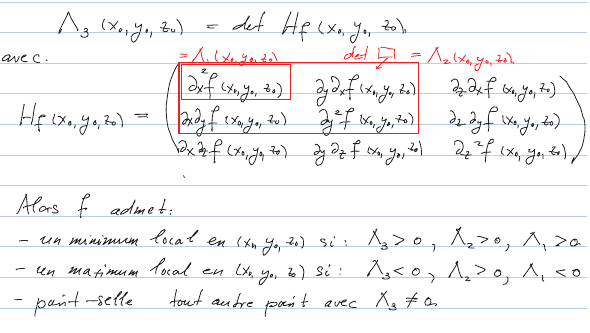
\includegraphics[scale=0.7]{cas_3}
	\caption{Le cas 3 variables}
\end{figure}
\subsection[Extremums liés]{Extremums liés (multiplicateurs de Lagrange)}
Le but est de trouver des extremums d'une fonction sous contrainte d'autres fonctions. Le cas typique est de trouver les dimensions d'un cylindre, qui maximisent le volume/minimisent la surface, donné la surface/le volume. Ce chapitre sera donc un exemple complet, avec des explications intermédiaires. Rappelons que la surface et le volume sont donnés par 
\begin{align*}
V-\pi r^2 h = g(r,h)\\
S = 2\pi r^2 + 2\pi rh = f(r,h)
\end{align*} Nous cherchons le les dimensions qui minimisent la surface, lorsque le volume V nous est donné. Deux méthodes s'offrent à nous : \\
\evid{Méthode 1:} Éliminer une variable : $h =  \frac{V}{\pi r^2}$ (la contrainte)
\begin{flalign*}
	S(r) &= f\(r,\frac{V}{\pi r^2}\) = 2\pi r^2 + 2\pi r\frac{V}{\pi r^2} = 2\pi r^2 + \frac{2V}{r}\\
	S'(r) &= 0 = 4\pi r - \frac{2V}{r^2} \to r = \(\frac{V}{2\pi}\)^{\frac{1}{3}}
\end{flalign*}
\evid{Méthode 2} Fonction de Lagrange :\\
Soit $\lambda \in \R$ et soit 
\[F(r,h,\lambda) = f(r,h) - \lambda\cdot g(r,h)\]
On cherche les points stationnaires de F, définis par $\nabla F = 0$
\begin{flalign*}
	F(r,h,\lambda) &= 2\pi r^2 + 2\pi r h - \lambda(V-\pi r^2 h)\\
	\nabla F(r,h,\lambda) &= \(\underbrace{4\pi r + 2\pi h - 2\pi r \lambda h}_{ =0,\ \circled{1}}\, , \, \underbrace{2\pi r + \lambda \pi r^2}_{=0, \circled{2}}, ,\, \underbrace{\pi r^2 h - V}_{=0, \circled{3}}\)^T
\end{flalign*}
Et on déduis nos valeurs depuis ces équations : \\
$\begin{array}{ll}
\circled{2}	& \to \lambda = -\frac{2}{r}\\
\circled{1}	& \to 4\pi r + 2\pi h - 2\pi r \frac{2}{r} \cdot h = 0 \to 4\pi r - 2\pi h = 0 \to h = 2r\\
\circled{3} &\to \pi r^2 2 r = V \to  r = \(\frac{V}{2\pi}\)^{\frac{1}{3}} \to \text{comme vu à la méthode 1}
\end{array}$\\
Cela se fait avec le théorème suivant : (attention aux conditions) \\
\evid{Théorème} (condition nécessaire pour un extremum)\\
Soient les fonctions $f,g : D \to \R,\ D\ \subset \R^2$ ouvert, $f,g$ de classe $C^1$. Si $f$ admet un extremum en $(x_0,y_0) \in D$ sous la contrainte $g(x_0,y_0) = 0$ \uline{et si $\nabla g(x_0,y_0) \neq 0$} alors il existe une valeur $\lambda_0$ telle que la fonction de Lagrange
\begin{equation*}
	F(x,y,\lambda) = f(x,y) - \lambda g(x,y)
\end{equation*}
soit stationnaire en $(x_0,y_0,\lambda_0)$\\
\\
Cela se teste de la manière suivante : calculer sous quelles conditions le gradient de $g$ vaut 0 (pour trouver  $(x_0,y_0)$. Si, avec ces valeurs, $g(x_0,y_0) = 0$ alors la méthode ne marche pas. Possible de le faire dans l'autre sens (chercher avec g et vérifier avec le gradient)

\subsection{Maximum/minimum absolus}
\begin{enumerate}[label=\roman*)]
	\item 	On localise les points stationnaires de $f$ à l'intérieur de $D$ $(g(\textbf{x}) < 0)$
	\item 	on localise les points où $g(\textbf{x}) = 0$ et $\nabla g(\textbf{x}) = 0$ (voir le contre exemple de la section 5.8.2)
	\item 	on localise les points stationnaires de la fonction de Lagrange \big($F(\textbf{x},\lambda) = f(\textbf{x}) - \lambda g(\textbf{x})\big)$
	\item 	On évalue $f$ aux points trouvés aux $i) \to iii)$ et compare les valeurs.
\end{enumerate}

\section{Intégrales multiples}
Attention à la notation : Les intégrales se lisent linéairement depuis l'intérieur. Explication : 
\[\int_0^1\int_5^9 3x^2 + 4y \deriv{x}\deriv{y}\]
Doit se lire de cette manière : 
\[\int_0^1\(\int_5^9 3x^2 + 4y \deriv{x}\)\deriv{y}\]
ou encore, afin d'éviter les confusions 
\[\int_0^1 \deriv{y}\int_5^9 \deriv{x}\ 3x^2 + 4y\]
La méthode d'intégration est très simple. On intègre selon une des variables, on l'évalue aux bornes données (si elles le sont), puis on répète pour les autres variables.
\subsection{Théorèmes, définitions}
\begin{itemize}
	\item 	Toute fonction continue sur un domaine D (borné et fermé) est intégrable sur D
	\item 	L'ordre d'intégration n'a pas d'importance, du moment que la fonction à intégrer est continue (théorème de Fubini)
\end{itemize}

\subsection{Domaines d'intégration}
La partie subtile du chapitre. Il faut bien comprendre sur quel domaine (pour des domaines complexes) on intègre. Voici des exemples :
\begin{figure}
	\centering
	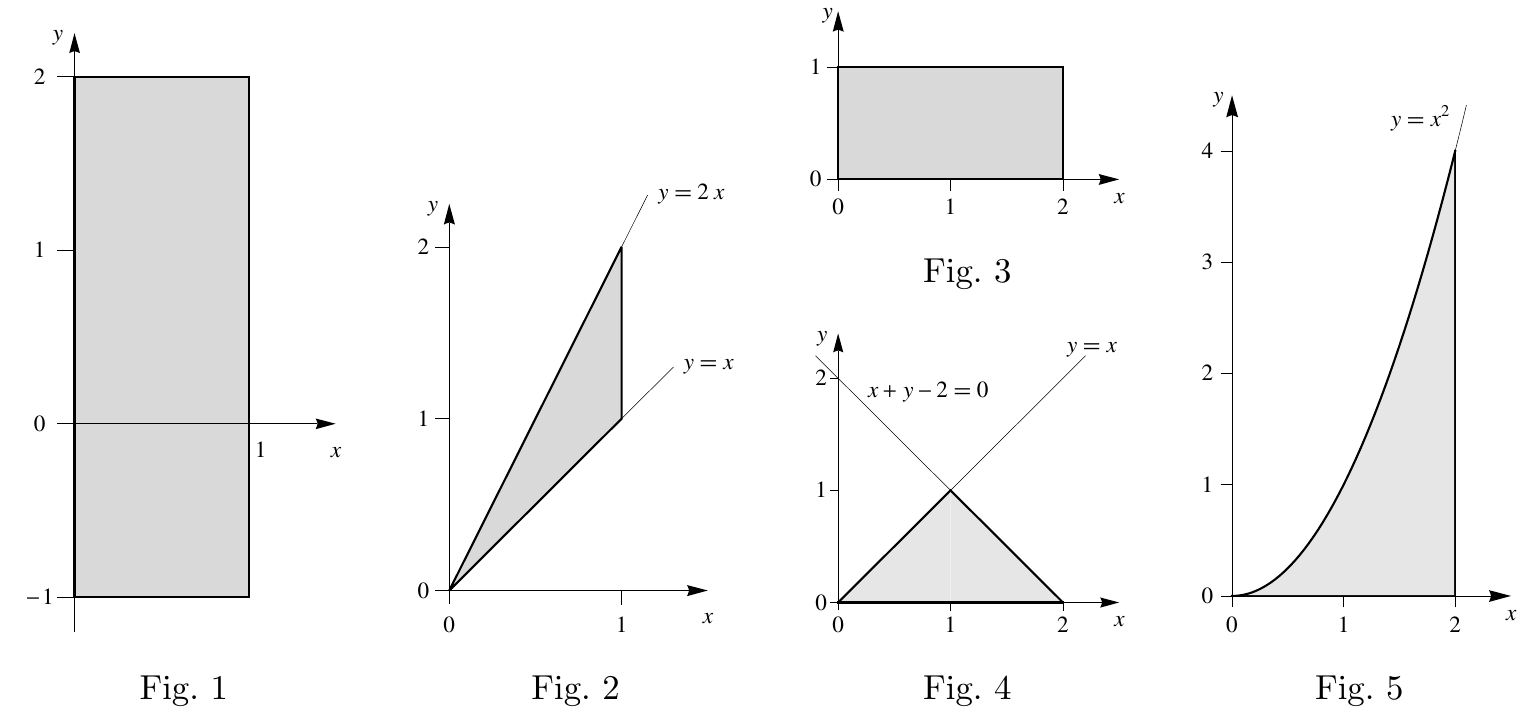
\includegraphics[scale=0.45]{domaine}
\end{figure}
\begin{itemize}
	\item 	Figure 1 : $\int_{-1}^2\int_0^2 f(x,y) \deriv{x}\deriv{y}$
	\item 	Figure 2 : $\int_0^1 \int_x^{2x} f(x,y) \deriv{y}\deriv{x}$
	\item 	Figure 3 : $D = \{(x,y) : 0 \leq x \leq 2,\ 0 \leq y \leq 1\} \iff \int_0^2 \int_0^1 f(x,y) \deriv{y}\deriv{x}$
	\item 	Figure 4 : $D = \{(x,y) : 0 \leq y \leq x,\ x+y-2 \leq 0\} \iff \int_0^1\int_0^x f(x,y) \deriv{y}\deriv{y} + \int_1^2\int_0^{2-x} f(x,y) \deriv{y}\deriv{x}$
	\item 	Figure 5 : $D = \{(x,y) : 0 \leq y \leq x^2,\ 0 \leq x \leq 2\} \iff \int_0^2 \int_0^{x^2} f(x,y) \deriv{y}\deriv{x}$
\end{itemize}
Notons qu'à la figure 4, nous nous sommes permis de séparer l'intégrale en deux parties. En effet, pour intégrer simplement, nous avons fait un dessin et constaté que $x$ allait bien de 0 à 2, mais y n'est pas défini par une droite fixe. Ainsi, il est plus simple de diviser en deux parties : la première ou x est entre 0 et 1, et y est délimité par $y=x$, et une deuxième où x est entre 1 et 2, et y est délimité par $y = 2-x$. Il est possible de le faire par calcul, mais la méthode du dessin reste la plus simple.	
\subsection{Changement de variables}
 Soit $G : \underset{\xi, \eta}{\overline{D}} \to \underset{x,y}{D}$, bijectif de classe $C^1$.\\
\begin{flalign*}
	(x,y)\ =&\ G(\xi,\eta) =  \big(G_1(\xi, \eta),\ G_2(\xi,\eta)\big)\\
	\overline{f}(\xi,\eta)\ =&\ f\big(G(\xi,\eta)\big)
\end{flalign*}
	\[
	\det(J_G(\xi,\eta)\ =\ \det
	\begin{pmatrix} 
		\frac{\delta G_1}{\delta \xi}(\xi,\eta) & \frac{\delta G_1}{\delta \eta}(\xi,\eta)\\
		\frac{\delta G_2}{\delta \xi}(\xi,\eta) & \frac{\delta G_2}{\delta \eta}(\xi,\eta)
 	\end{pmatrix}
 	\]
 Alors 
	 \begin{boite}[0.5]
	 	\[\int\limits_D f(x,y) \deriv{x}\deriv{y} = \int\limits_{\overline{D}} \overline{f}(\xi,\eta)\ \big|\det(J_G(\xi,\eta)\big| \deriv{\xi}\deriv{\eta}\]
	 \end{boite}	
En notant $det(J_G(\xi,\eta)$ := le jacobien du changement de variables. La relation entre une matrice d'un changement G et la matrice du changement inverse est noté par $H = G^{-1}$. Autrement dit, trouver le changement de variables inverse se calcule avec l'inverse de la jacobienne. De la même manière, sans devoir calculer cette inversion, on note que 
\[
	\det\big(J_H(x,y)\big) = \left[\frac{1}{\det\big(J_G(\xi,\eta)\big)}\right]_{(\xi,\eta) = H(x,y)}
\]
\begin{exemple}
	Prenons le cas des coordonnées polaires. L'application G est alors définie par 
	\[G(r,\varphi) = \big(r\cos(\varphi),r\sin(\varphi)\big)\]
	Sa jacobienne est naturellement
	\[
	J_G(r,\varphi)  =	
	\begin{pmatrix}
		\cos(\varphi) & -r\sin(\varphi)\\
		\sin(\varphi) & r\cos(\varphi)
	\end{pmatrix}
	\]
	et son Jacobien (son déterminant) par 
	\[
		\det J_G(r,\varphi) =  r\cos(\varphi)^2 + r\sin(\varphi)^2 = r
	\]
	Calculer le Jacobien de H semble maintenant complexe et long. Mais comme, par définition, $H = G^{-1}$, la jacobienne de H est simplement l'inverse de celle de G mais évaluée en $(r,\varphi) = \big(H_1(x,y),H_2(x,y)\big)$. En sachant que l'opération inverse est définie par $r = \sqrt{x^2 + y^2}$, la relation entre les jacobien est 
	\[
		\det\big(J_H(x,y)\big) = \left[\frac{1}{\det\big(J_G(r,\varphi)\big)}\right]_{(r,\varphi) = H(x,y)} = \left[\frac{1}{r}\right]_{r = \sqrt{x^2 + y^2}} = \frac{1}{\sqrt{x^2 + y^2}}
	\]
\end{exemple}
\begin{exemple}
	Calcul de l'aire d'un cercle de rayon R avec un changement de variables :\\
	On peut calculer avec les coordonnées cartésiennes, mais ce serait long et embêtant. Au lieu de ça, nous pouvons calculer avec les coordonnées polaires, comme définies au dessus. Ainsi :
	\[\text{aire(}C_R) = \iint_{C_R} \deriv{x}\deriv{y} = \int_0^R \int_0^{2\pi} r\deriv{\varphi}\deriv{r} = 2\pi\int_0^R r \deriv{r} = 2\pi \left[\frac{1}{2}r^2\right]_0^R = \pi R^2\]
	Notons aussi que le passage à la deuxième dérivée s'est fait grâce à l'information que le jacobien de G est $r$
\end{exemple}
\begin{exemple}
	Calculer l'intégrale de \[\iint_D x^3y^3 \deriv{x}\deriv{y}\]
	sur le domaine délimité par les courbes
	\[\left\{\begin{array}{l}
	x^2 + y^2 = 5\\
	x^2 + y^2 = 9\\
	x^2 - y^2 = 1\\
	x^2 - y^2 = 4
	\end{array}\right.
	\]
	Le calcul direct (même avec séparation du domaine) se fait de manière très compliquée. Le mieux reste de faire un changement de variables, en identifiant un couple $u,v$ qui correspond. Une manière de faire est de prendre $(u,v) = (x^2+y^2,\ x^2-y^2)$ Nous pouvons donc calculer le nouveau domaine : $\overline{D} = [5,9]\times [1,4]$ et la Jacobienne de $H : \begin{pmatrix}
	2x & 2y\\
	2x & -2y
	\end{pmatrix}$ qui nous donne directement son déterminant : $\det J_H = -8xy$ et celui de G \[\det J_G =[\det J_H^{-1}]_{x,y = G(u,v)} = \left[\frac{-1}{8xy}\right]_{(x,y) = G(u,v)}\]
	et donc 
	\begin{align*}
	\iint_D x^3y^3 \deriv{x}\deriv{y} = \iint_{\overline{D}} [x^3y^3]_{G(u,v)} |\det J_G(u,v)| \deriv{u}\deriv{v} = \frac{1}{8}\iint_{\overline{D}} \left[y^3y^3\cdot\frac{1}{xy}\right]_{G(u,v)}\deriv{u}\deriv{v}\\
	\end{align*}
	Et nous devons maintenant remplacer $x,y$ par des fonctions de $u,v$ (nous notons rapidement que $u+v = 2x^2$ et $u-v = 2y^2$). Nous remplaçons également $\overline{D}$ par ce qu'il est $\(\int_1^4\int_5^9 [\ldots] \deriv{u}\deriv{v}\)$ et le reste de l'intégrale n'est plus que formalité.
	
	Pour le développement complet, série 13 exo 2 i)
\end{exemple}

\subsection{Centre de gravité}
Soit $g(x,y,z) > 0$ une fonction donnant la distribution de masse du domaine D. Nous calculons
\[\left\{\begin{array}{l}
I = \int_D g(x,y,z) \deriv{x}\deriv{y}\deriv{z}\\
I_1 = \int_D xg(x,y,z) \deriv{x}\deriv{y}\deriv{z}\\
I_2 = \int_D yg(x,y,z) \deriv{x}\deriv{y}\deriv{z}\\
I_3 = \int_D zg(x,y,z) \deriv{x}\deriv{y}\deriv{z}\\
\end{array}\right.\]
Le centre de gravité de cette fonction est placé en
\[\(\frac{I_1}{I},\frac{I_2}{I},\frac{I_2}{I}\)\]
Notons que si la distribution de masse est constante (g est une fonction constante), on peut prendre g = 1.

\subsection{Quelques choses à savoir}
\begin{itemize}
	\item 	Coordonnées sphériques : 
			$\left\{\begin{array}{l}
				x = r\sin(\theta)\cos(\varphi)\\
				y = r\sin(\theta)\cos(\varphi)\\
				z =\cos(\theta)
			\end{array}\right.$
			avec $0 \leq \theta \leq \pi$ qui tourne de haut en bas et $0\leq \varphi < 2\pi$ qui tourne autour de l'axe vertical.\\
			$J_G = 
			\begin{pmatrix}
				\sin(\theta)\cos(\phi) & r\cos(\theta)\cos(\phi) & -r\sin(\theta)\sin(\phi)\\
				\sin(\theta)\sin(\phi) & r\cos(\theta)\sin(\phi) & r\sin(\theta)\cos(\phi)\\
				\cos(\theta) & -r\sin(\theta) & 0
			\end{pmatrix} det(J_G(r,\theta,\phi) = r^2 \sin(\theta)$
	\item 	Coordonnées cylindriques
			$\left\{\begin{array}{l}
				x = r\cos(\varphi)\\
				y = r\sin(\varphi)\\
				z = z
			\end{array}\right. J_G(r,\varphi,z) = 
			\begin{pmatrix}
				\cos(\varphi) & -r\sin(\varphi) & 0\\
				\sin(\varphi) & r\cos(\varphi) & 0\\
				0 & 0 & 1
			\end{pmatrix} \\
			\det J_G(r,\varphi,z) = r$
\end{itemize}
\end{document}